\documentclass[9pt,a4paper]{article}
\usepackage[utf8]{inputenc}
\usepackage[T1]{fontenc}
\usepackage[spanish]{babel}
\usepackage[a4paper,margin=1.45cm]{geometry}
\usepackage{graphicx}
\usepackage{booktabs}
\usepackage{amsmath}
\usepackage{float}
\usepackage[hidelinks]{hyperref}
\usepackage{caption}
\usepackage{array}
\usepackage{microtype}

\graphicspath{{figures/}}
\setlength{\parindent}{0pt}
\setlength{\parskip}{0.28em}
\setlength{\floatsep}{4pt}
\setlength{\textfloatsep}{4pt}
\setlength{\intextsep}{4pt}
\captionsetup{font=small,labelfont=bf}

\title{Segmentación de miotubos en imágenes de microscopía\\[-2mm]
\large Informe de EDA y resultados experimentales}
\author{Proyecto myotubes-seg}
\date{20 de noviembre de 2026}

\begin{document}
\maketitle

\section{Objetivo y datos}

El objetivo fue preparar el conjunto \texttt{vt} y comparar métodos de segmentación binaria. Se evaluaron dos líneas base en validación y dos variantes YOLOv11-seg. El conjunto de prueba quedó reservado.

El inventario tiene 306 imágenes, de 2592 por 1944 píxeles aproximadamente. Los miotubos ocupan solo el 1.759\% del área anotada, con 2148 instancias. Las imágenes originales incluyen 34 máscaras vacías. La mediana de área por imagen es 0.861\%, con gran variación entre casos.

\begin{figure}[H]
\centering
\begin{minipage}[t]{0.49\textwidth}
\centering
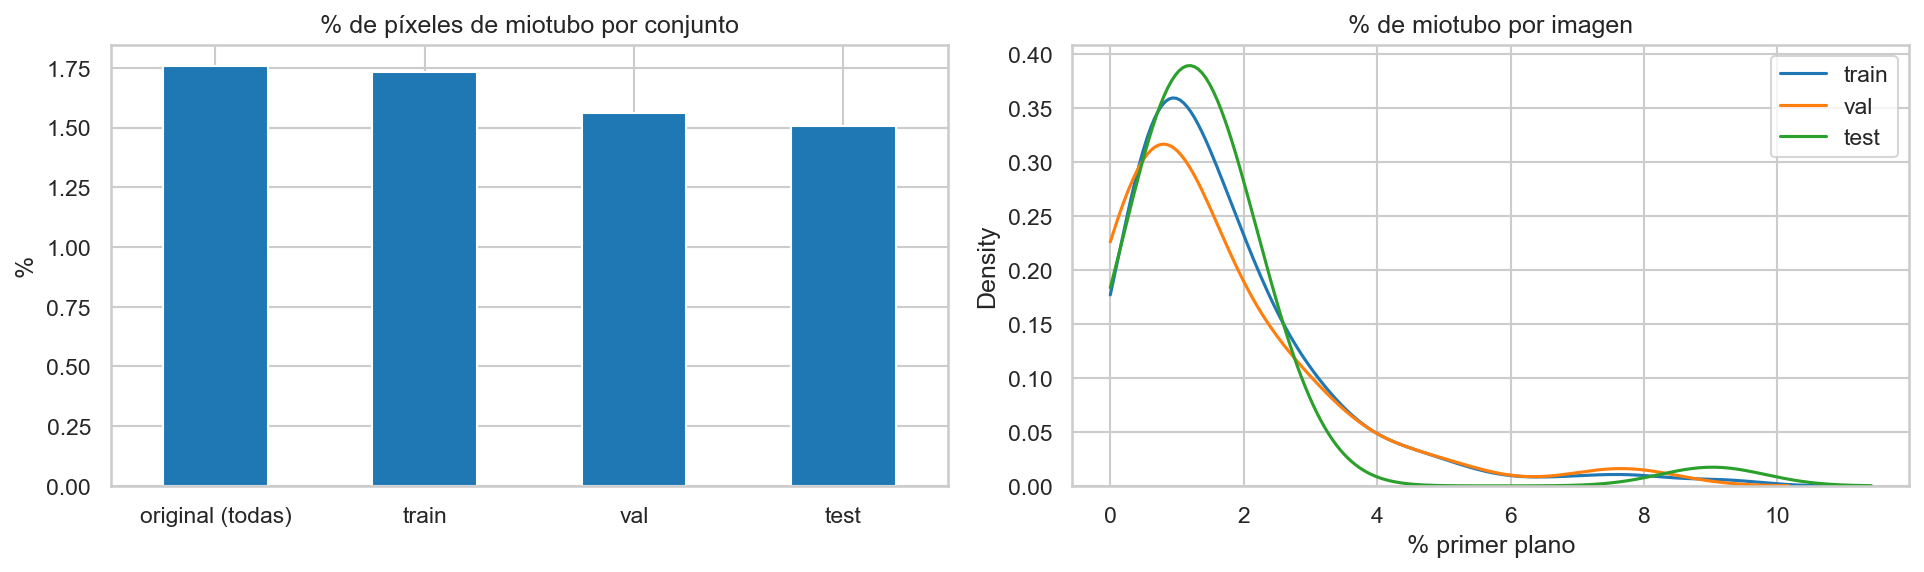
\includegraphics[width=\linewidth]{fig_desbalance.png}
\captionof{figure}{Desbalance de clases.}
\end{minipage}\hfill
\begin{minipage}[t]{0.49\textwidth}
\centering
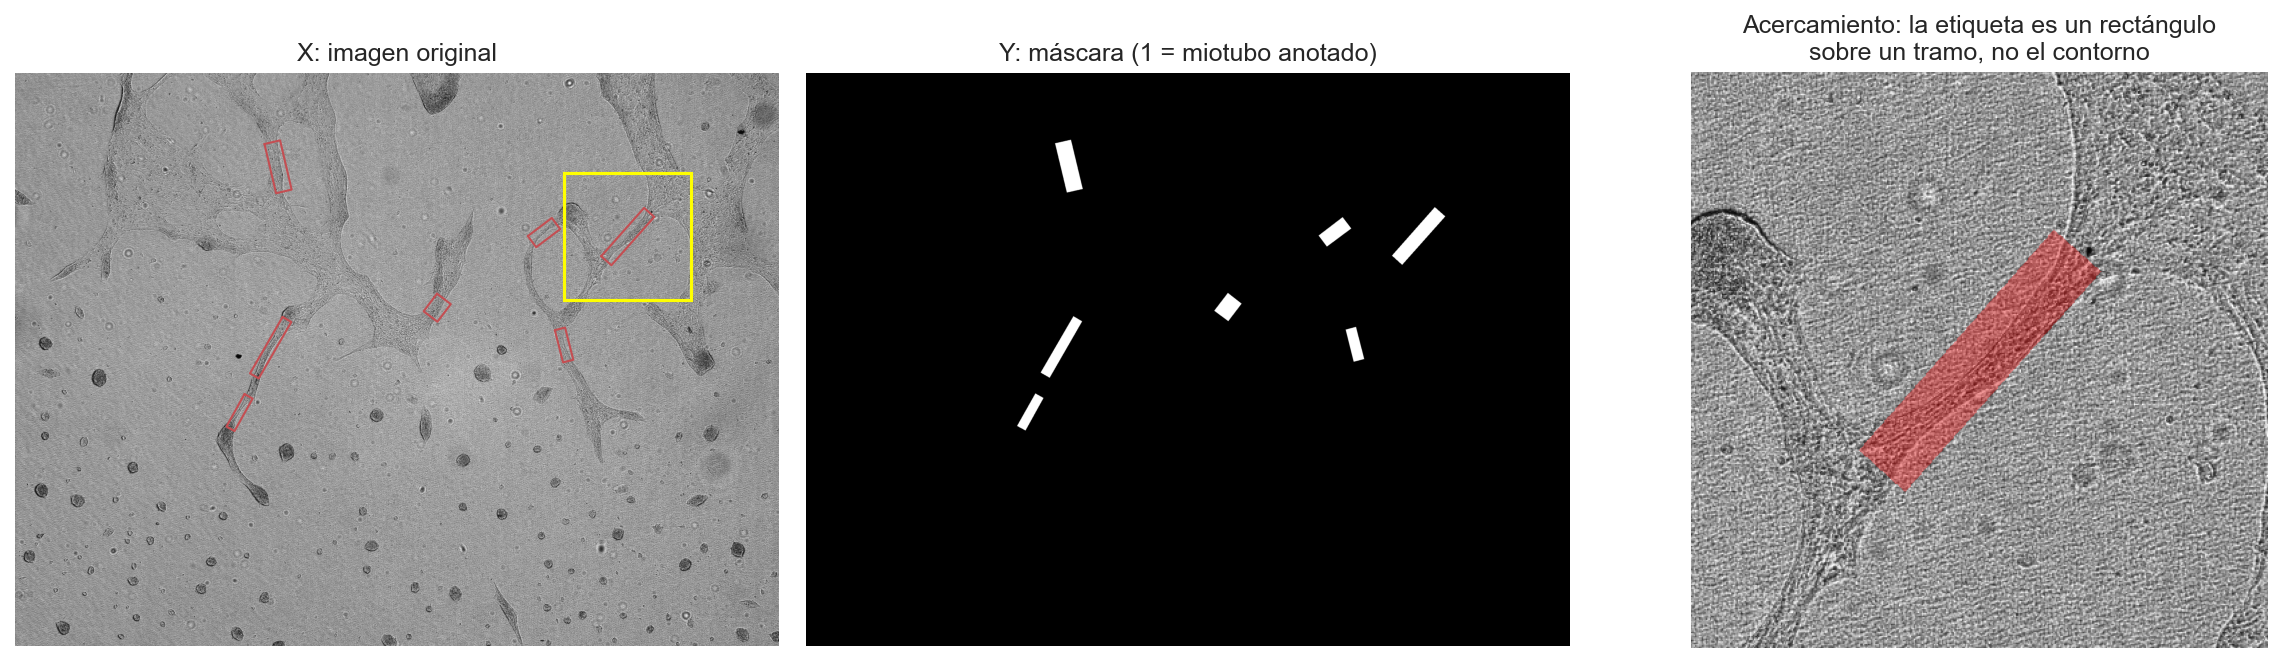
\includegraphics[width=\linewidth]{fig_etiqueta.png}
\captionof{figure}{Ejemplo de imagen y anotaciones.}
\end{minipage}
\end{figure}

Las máscaras YOLO y PNG son globalmente coherentes: mediana de IoU 0.9583. En 51 imágenes el IoU es menor a 0.95. También se encontraron 34 máscaras sin instancias, algunas con miotubos visibles, por lo que no pueden considerarse automáticamente como negativos reales.

\section{Fuga de datos y partición}

Se encontraron 117 pares casi duplicados, 16 idénticos y 54 clústeres con al menos dos copias. Una partición aleatoria produjo una fuga media de 36.2\% entre validación y entrenamiento, con un máximo de 56.5\% en 50 semillas.

La partición final agrupa duplicados y identificadores de célula. Esta estrategia produjo cero imágenes de validación duplicadas en entrenamiento. Se excluyeron máscaras vacías y cajas mayores al 20\% del área. Los grupos restantes se asignaron 70/15/15 con semilla 42.

\begin{table}[H]
\centering
\small
\caption{Tamaño y desbalance de las particiones.}
\begin{tabular}{lrrrrr}
\toprule
Conjunto & Imágenes & Instancias & Miotubo & Fondo/miotubo & Vacías\\
\midrule
Original & 306 & 2148 & 1.759\% & 55.84 & 34\\
Entrenamiento & 136 & 1144 & 1.734\% & 56.68 & 0\\
Validación & 30 & 218 & 1.563\% & 62.99 & 0\\
Prueba & 29 & 327 & 1.505\% & 65.45 & 0\\
\bottomrule
\end{tabular}
\end{table}

\begin{figure}[H]
\centering
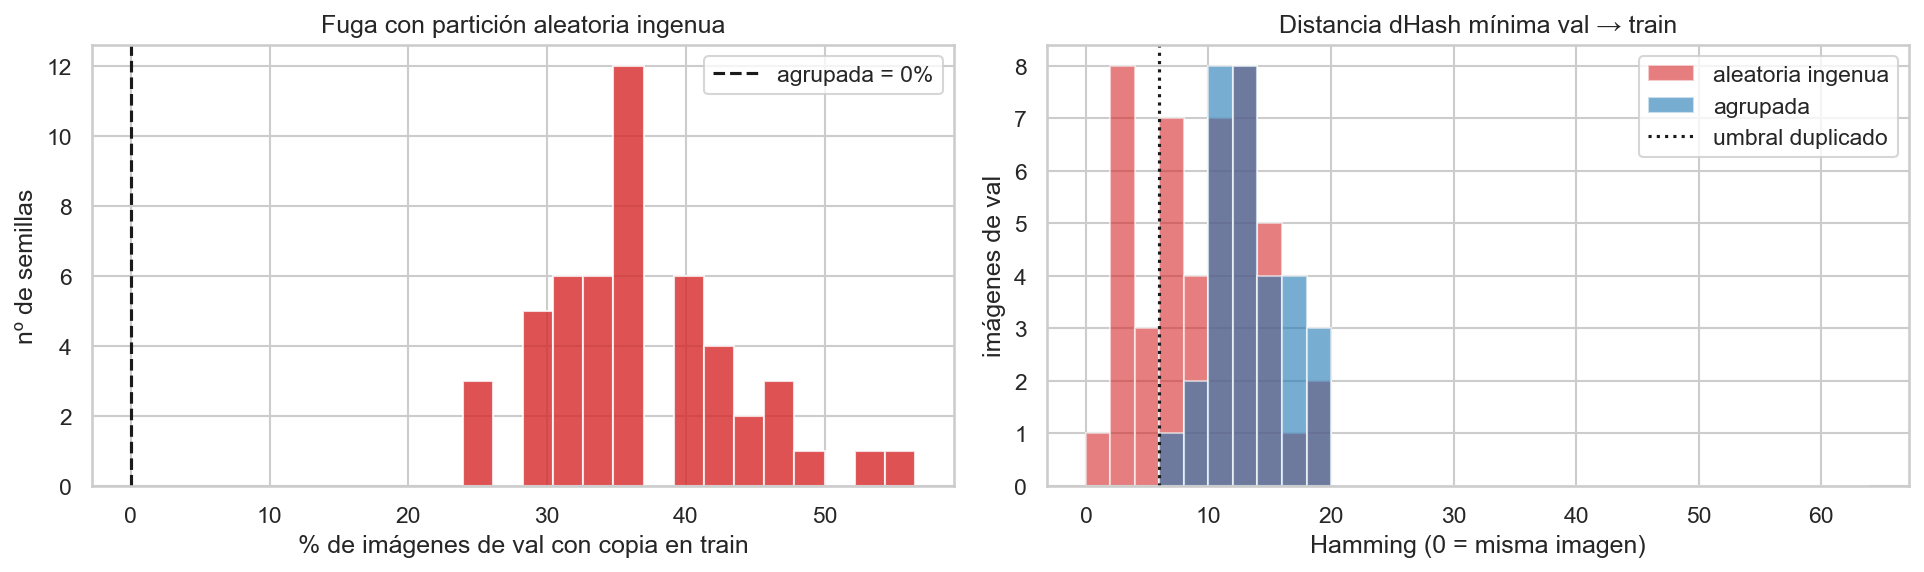
\includegraphics[width=0.62\textwidth]{fig_fuga.png}
\caption{Fuga en particiones aleatorias y agrupadas.}
\end{figure}

Las imágenes se particionaron en 136 para entrenamiento, 30 para validación y 29 para prueba. Las 74 imágenes descartadas por duplicado y las 37 excluidas se registraron para futuras referencias.

\section{Líneas base}

Se evaluaron dos métodos sin aprendizaje profundo a escala 0.25. Los umbrales se ajustaron solo con entrenamiento.

\begin{table}[H]
\centering
\small
\caption{Resultados sobre validación.}
\begin{tabular}{lrrrrr}
\toprule
Método & PR-AUC & ROC-AUC & IoU & Dice & Precisión\\
\midrule
Sato, umbral y morfología & 0.0666 & 0.7202 & 0.0831 & 0.1535 & 0.1008\\
Características y HGB & 0.1763 & 0.8968 & 0.1650 & 0.2832 & 0.3084\\
\bottomrule
\end{tabular}
\end{table}

La línea clásica alcanzó 0.3222 de recall con 0.1008 de precisión. El clasificador HGB obtuvo mejor PR-AUC, ROC-AUC, IoU y Dice. Su recall fue 0.2618 y su precisión 0.3084. Ningún método alcanzó precisión global de al menos 0.80 en validación. La prevalencia aleatoria fue 0.0156, frente a PR-AUC de 0.0666 y 0.1763.

\begin{figure}[H]
\centering
\begin{minipage}[t]{0.49\textwidth}
\centering
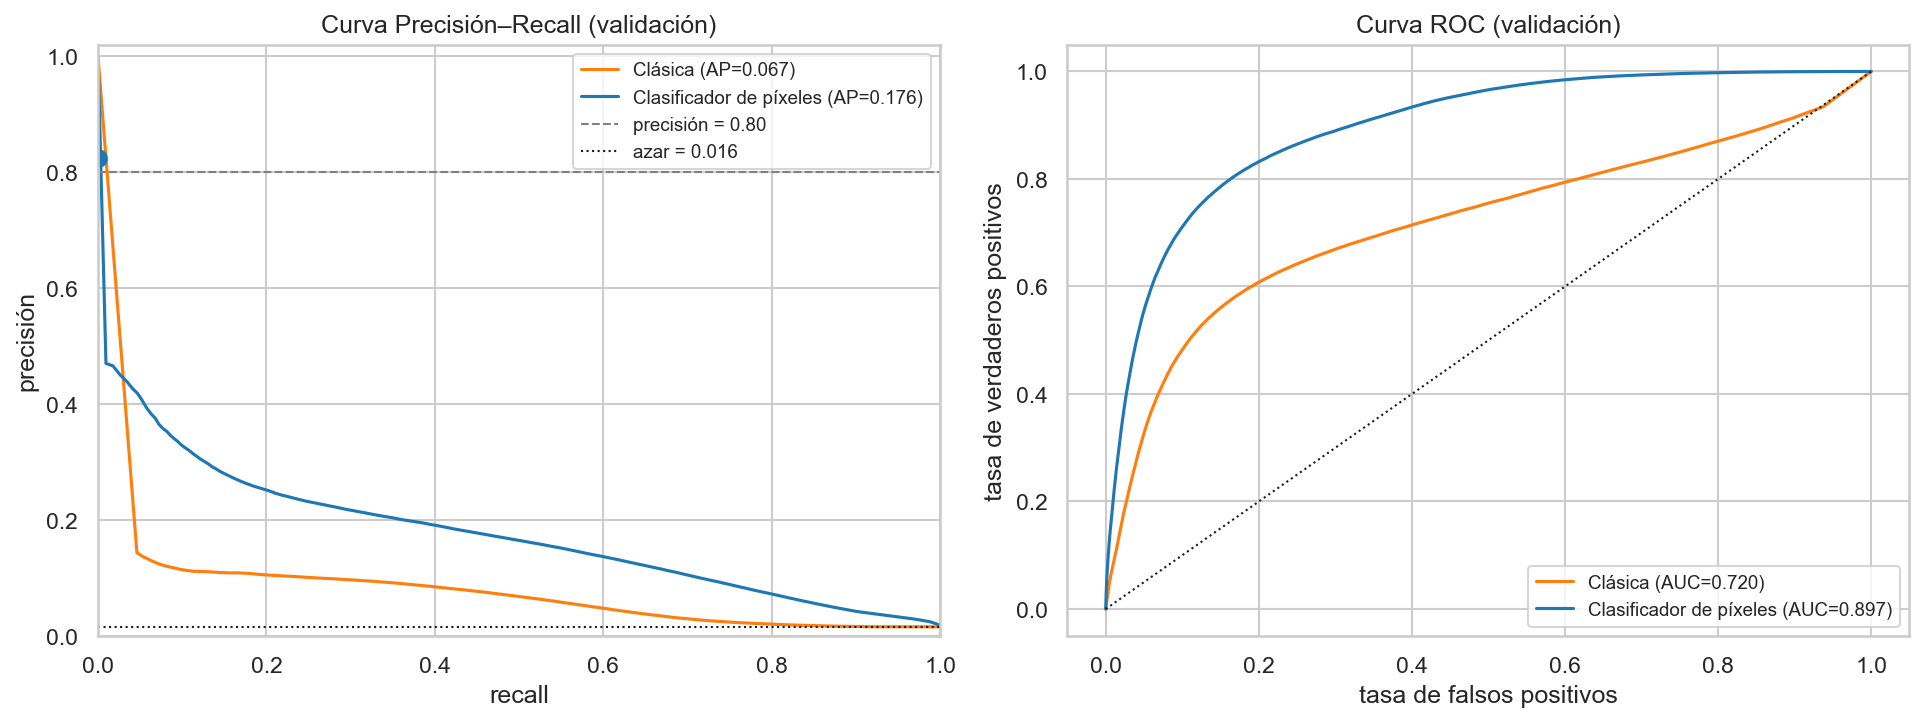
\includegraphics[width=\linewidth]{fig_pr_roc.png}
\captionof{figure}{Curvas PR y ROC.}
\end{minipage}\hfill
\begin{minipage}[t]{0.49\textwidth}
\centering
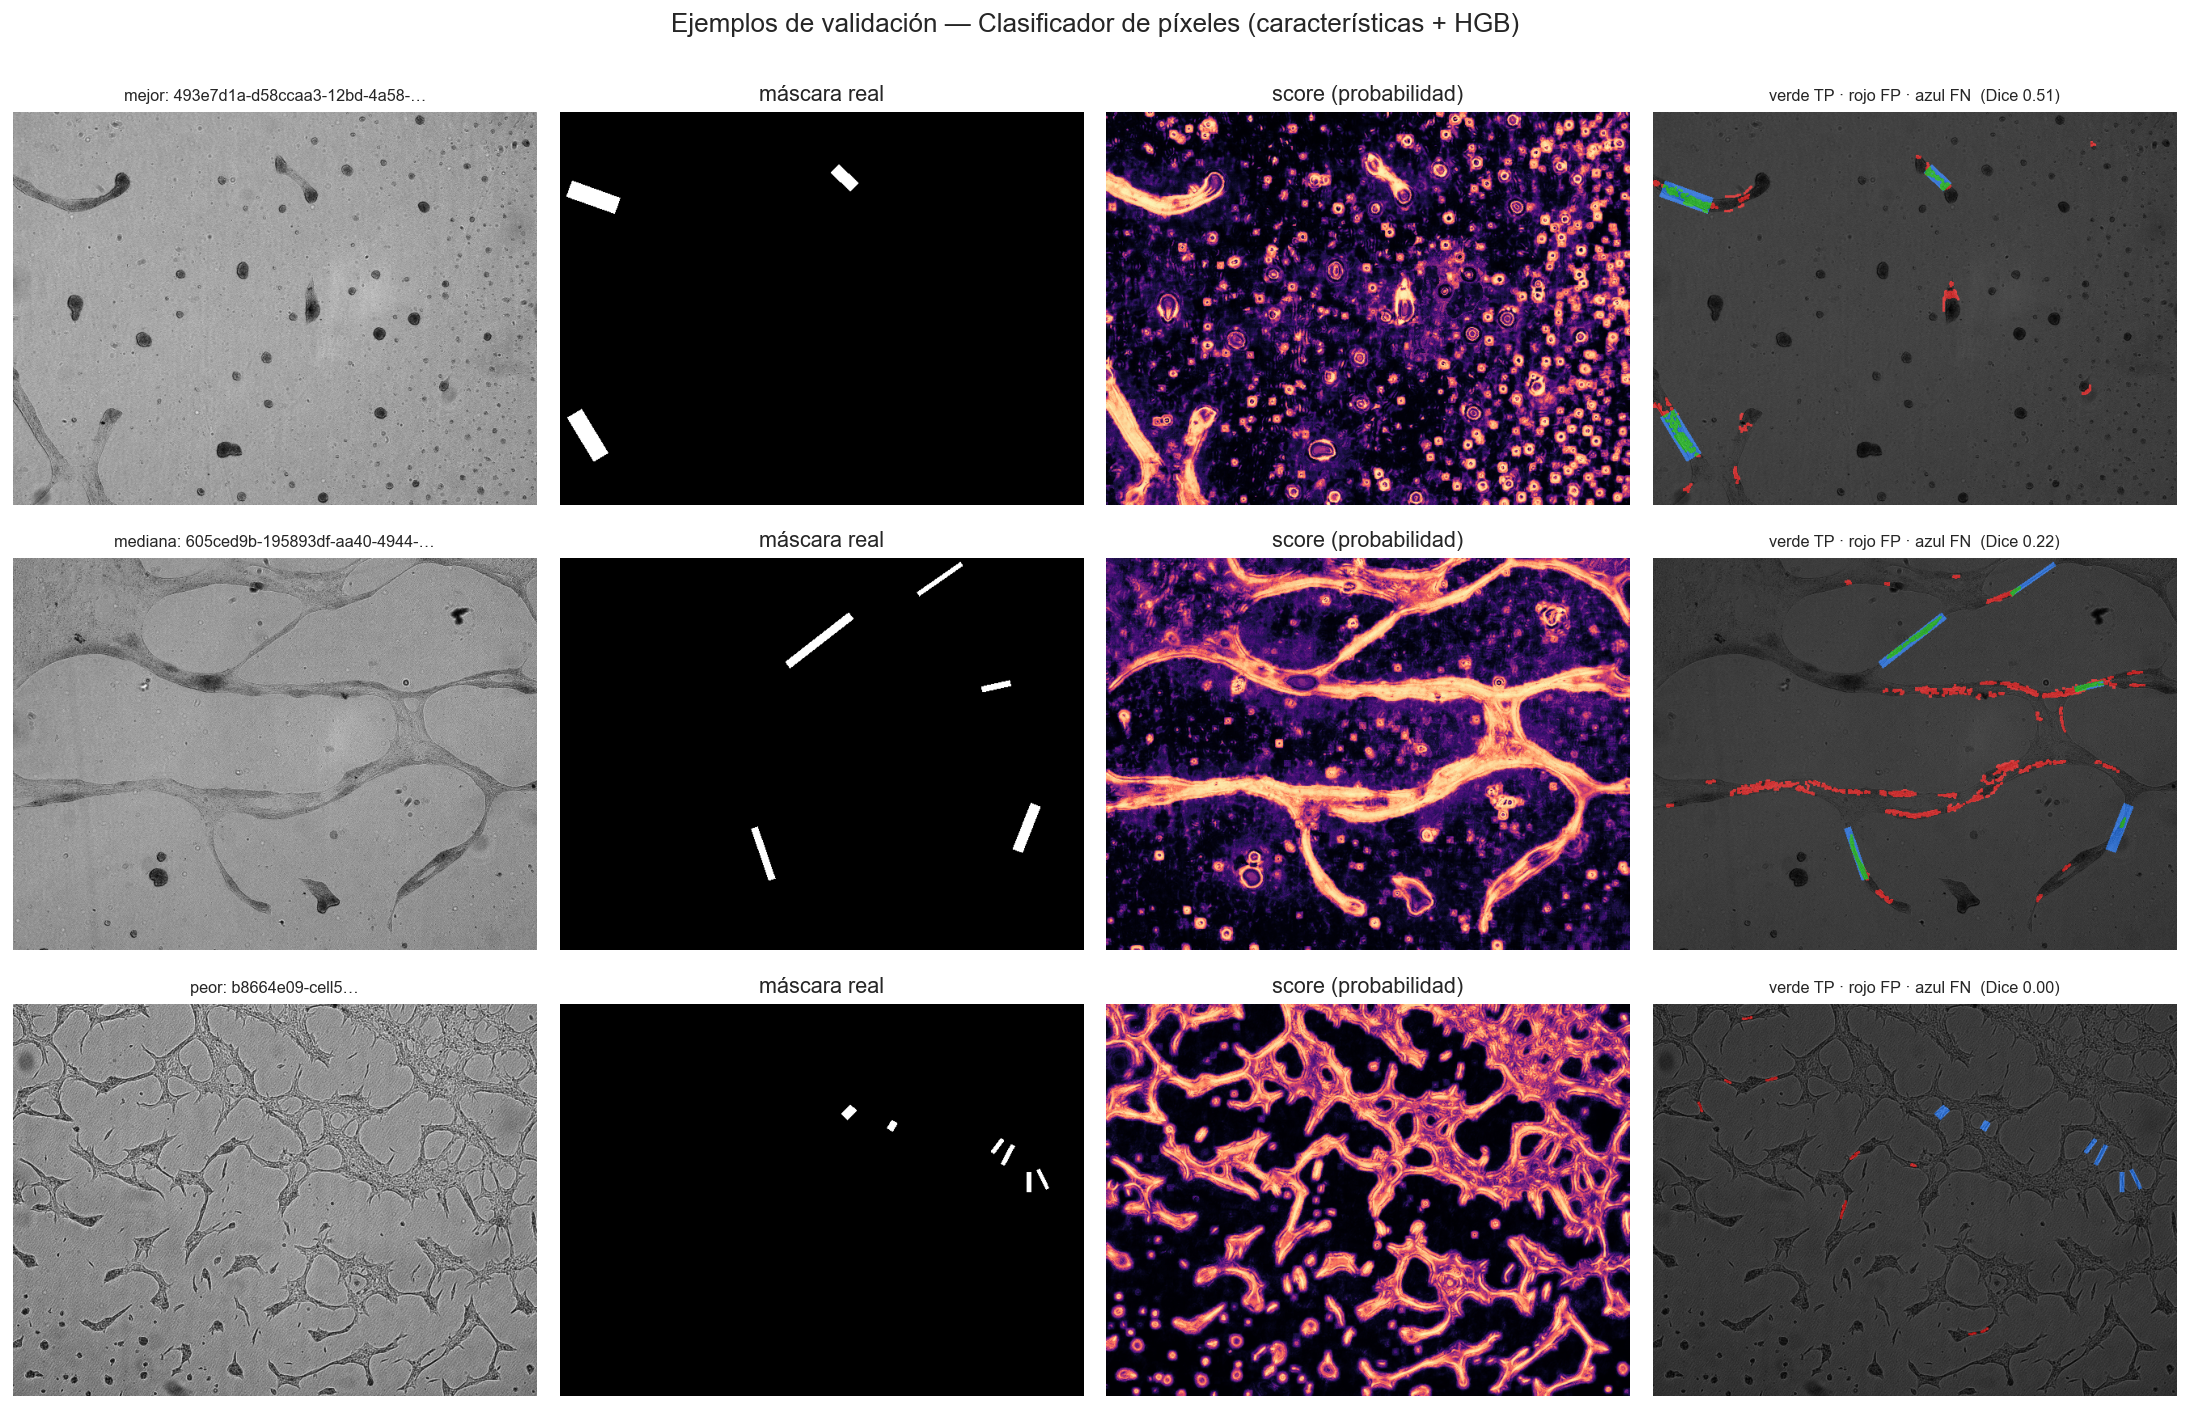
\includegraphics[width=\linewidth]{fig_cualitativo.png}
\captionof{figure}{Ejemplos cualitativos.}
\end{minipage}
\end{figure}

Las métricas por imagen presentan dispersión amplia. La zona de miotubo y las regiones anchas o finas muestran diferentes dificultades. El desbalance sigue limitando el rendimiento y puede sesgar las métricas globales a favor del fondo.

\section{Experimentos YOLOv11-seg}

Se probaron dos configuraciones durante 50 épocas, con resolución 1024, una clase y semilla 42. Transferencia congeló las primeras 10 capas. Fine-tune actualizó todos los parámetros.

\begin{table}[H]
\centering
\small
\caption{Máximos de máscara en validación.}
\begin{tabular}{lrrrr}
\toprule
Modelo & mAP50 & Época & mAP50-95 & Época\\
\midrule
Transferencia & 0.4364 & 50 & 0.1596 & 33\\
Fine-tune & 0.4763 & 48 & 0.1692 & 45\\
\bottomrule
\end{tabular}
\end{table}

Fine-tune supera a transferencia en ambos indicadores máximos. En su mejor época alcanzó precisión 0.4891 y recall 0.5379. Transferencia obtuvo 0.4574 y 0.4690 en la época 50.

\begin{figure}[H]
\centering
\begin{minipage}[t]{0.49\textwidth}
\centering
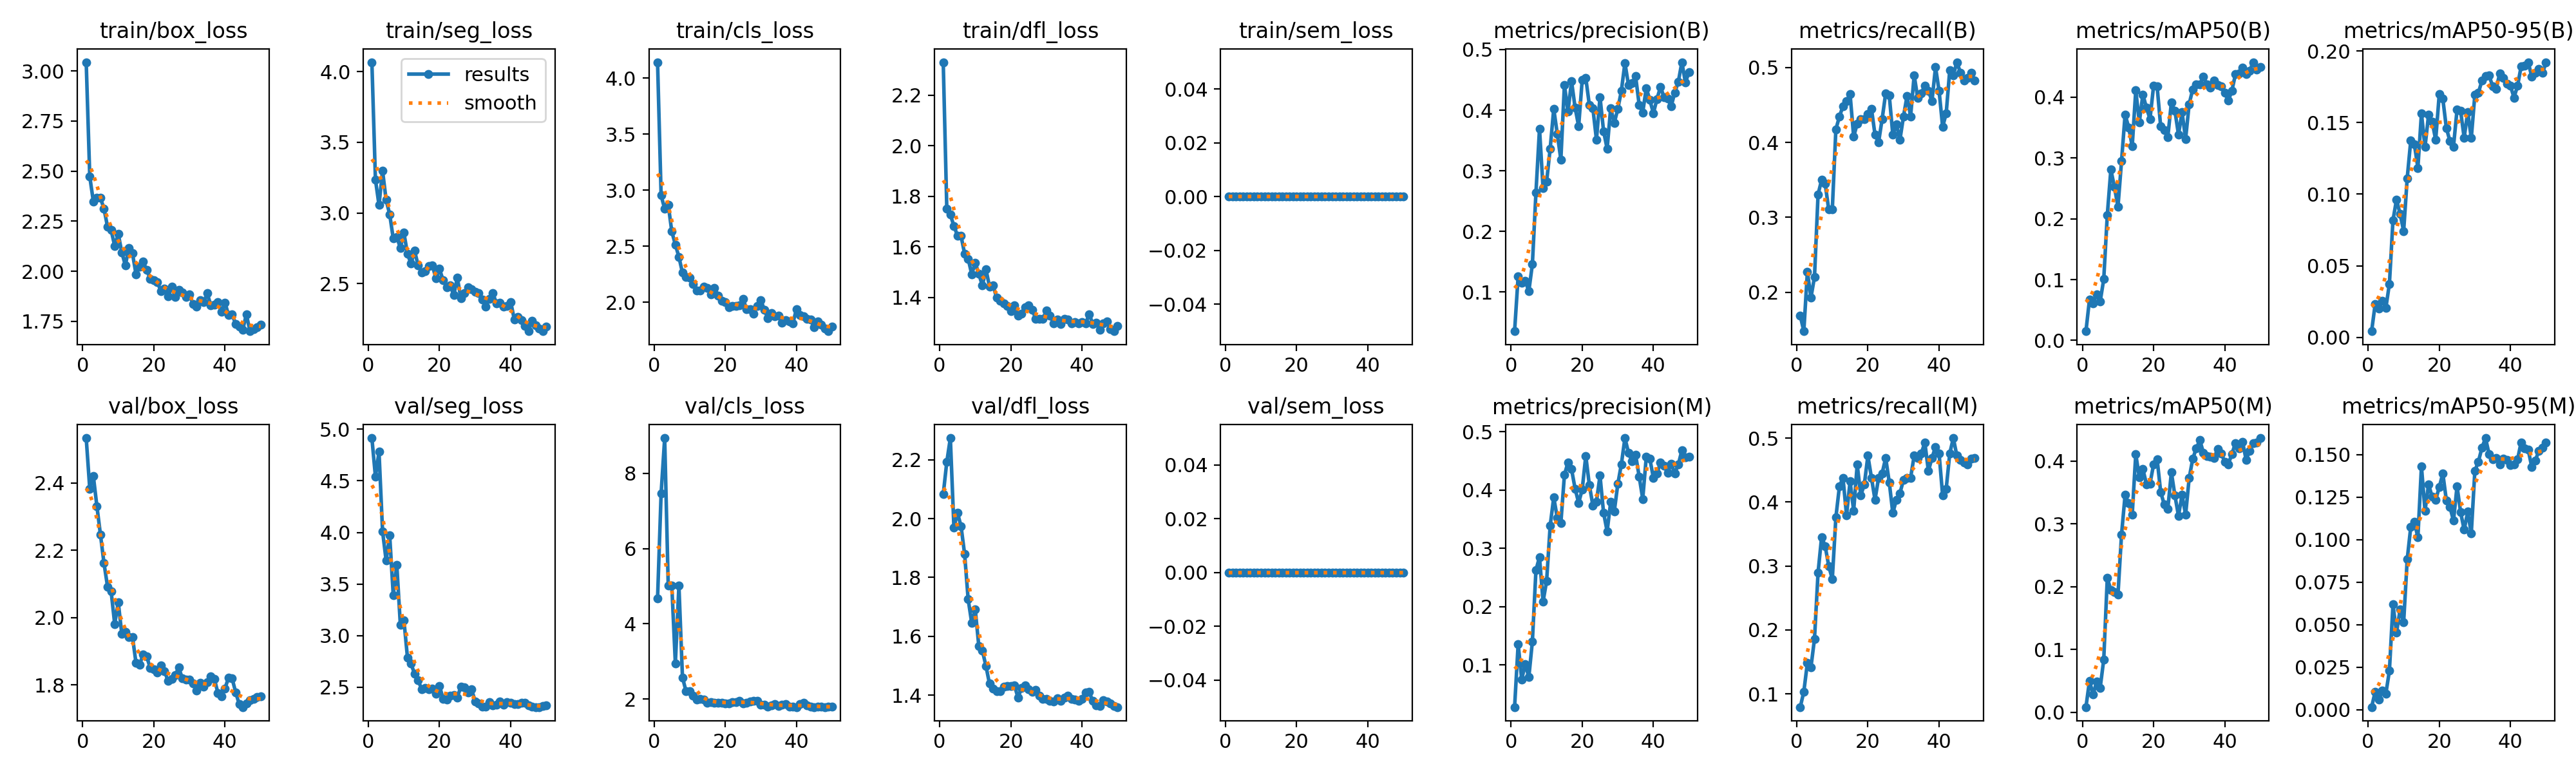
\includegraphics[width=\linewidth]{yolo_transfer_results.png}
\captionof{figure}{Transferencia.}
\end{minipage}\hfill
\begin{minipage}[t]{0.49\textwidth}
\centering
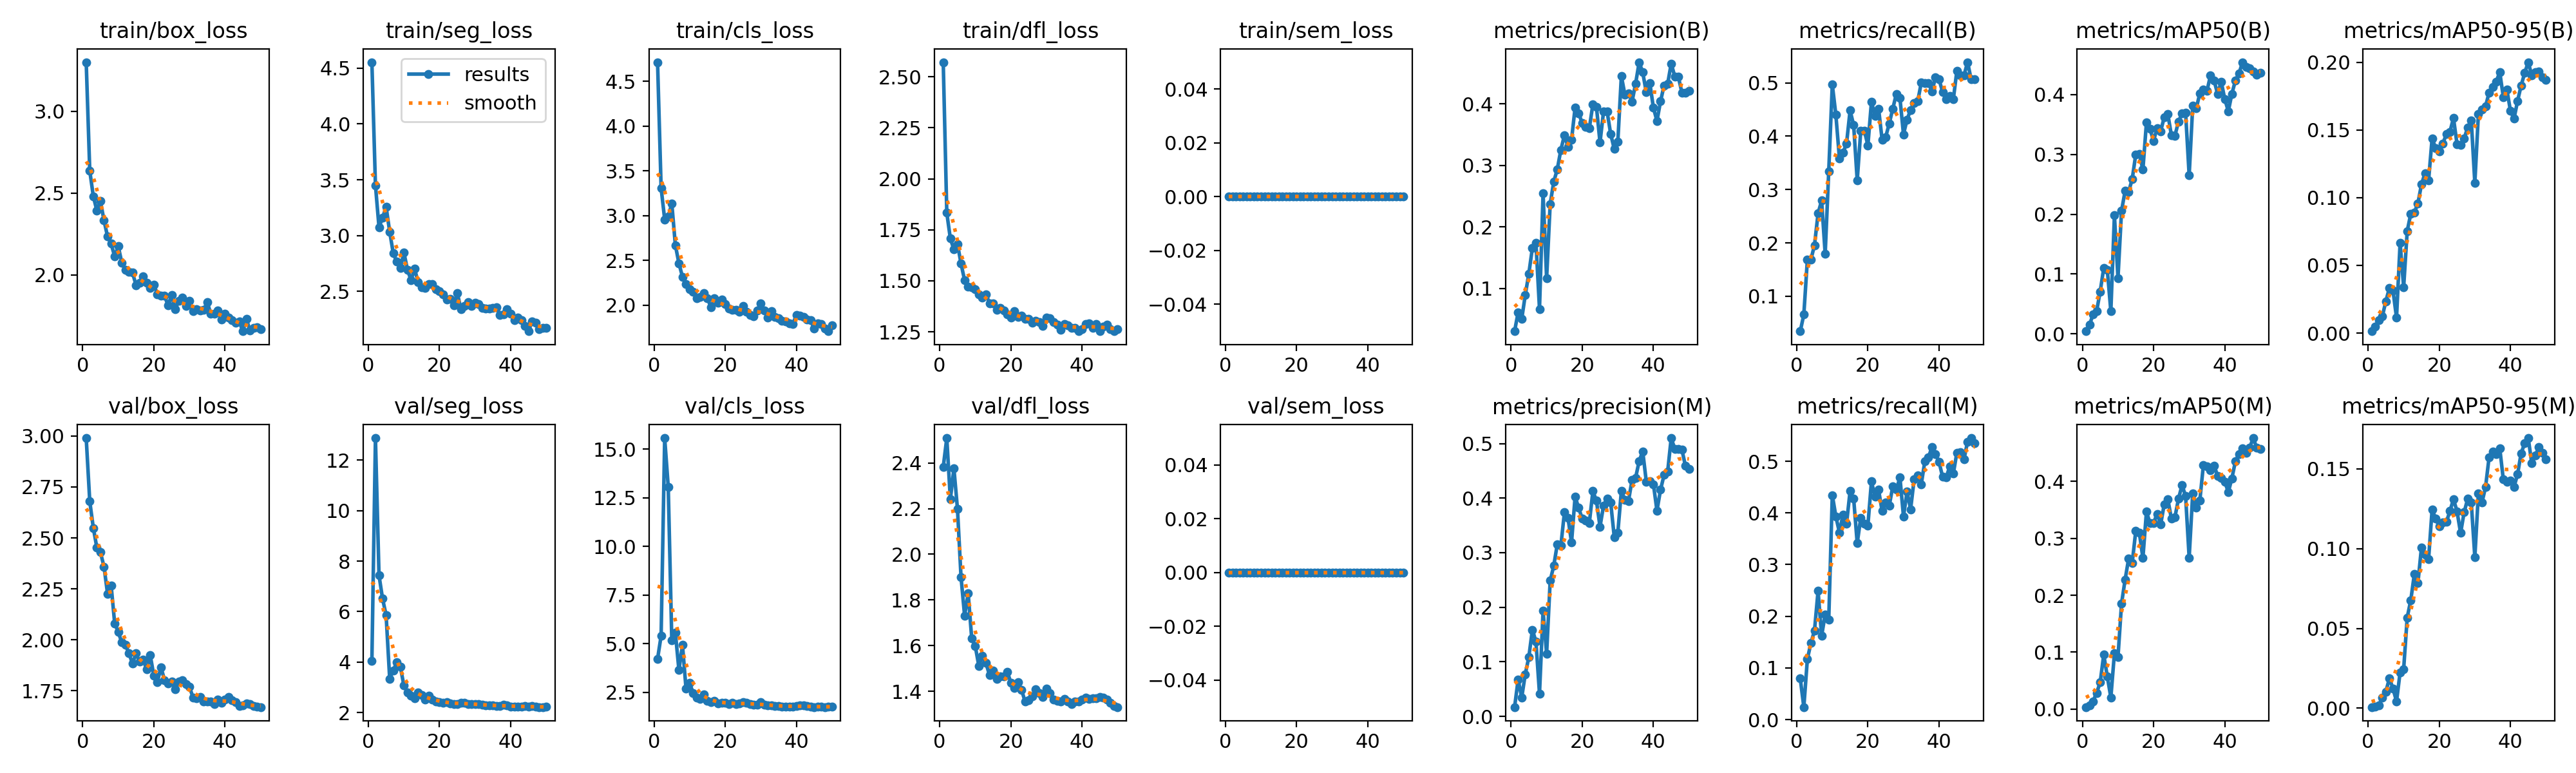
\includegraphics[width=\linewidth]{yolo_finetune_results.png}
\captionof{figure}{Fine-tune.}
\end{minipage}
\end{figure}

\begin{figure}[H]
\centering
\begin{minipage}[t]{0.49\textwidth}
\centering
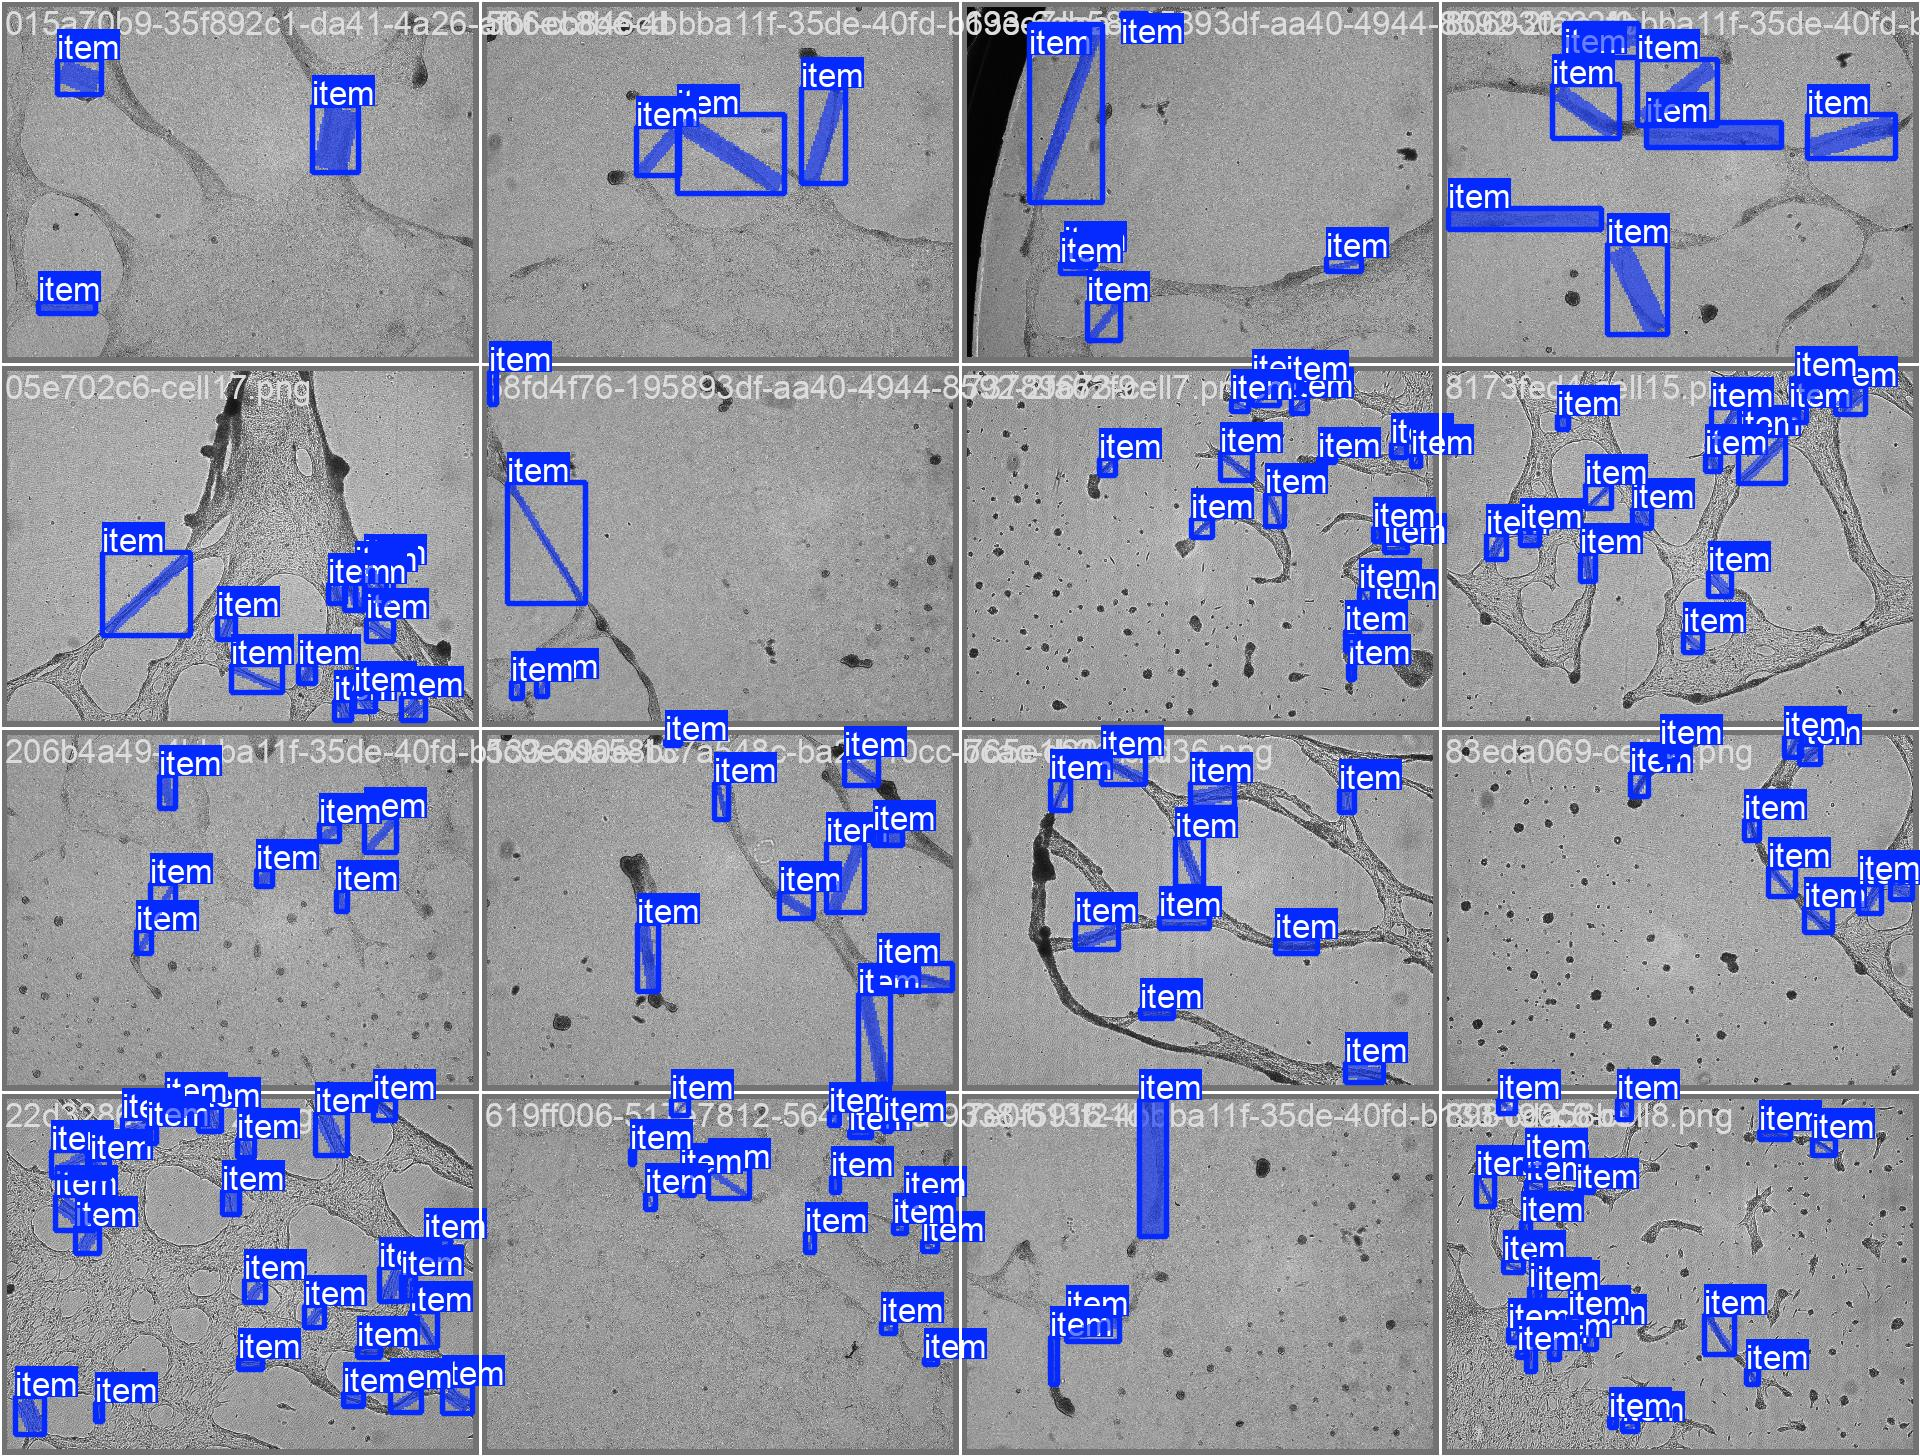
\includegraphics[width=\linewidth]{yolo_transfer_val_labels.jpg}
\captionof{figure}{Referencia YOLO.}
\end{minipage}\hfill
\begin{minipage}[t]{0.49\textwidth}
\centering
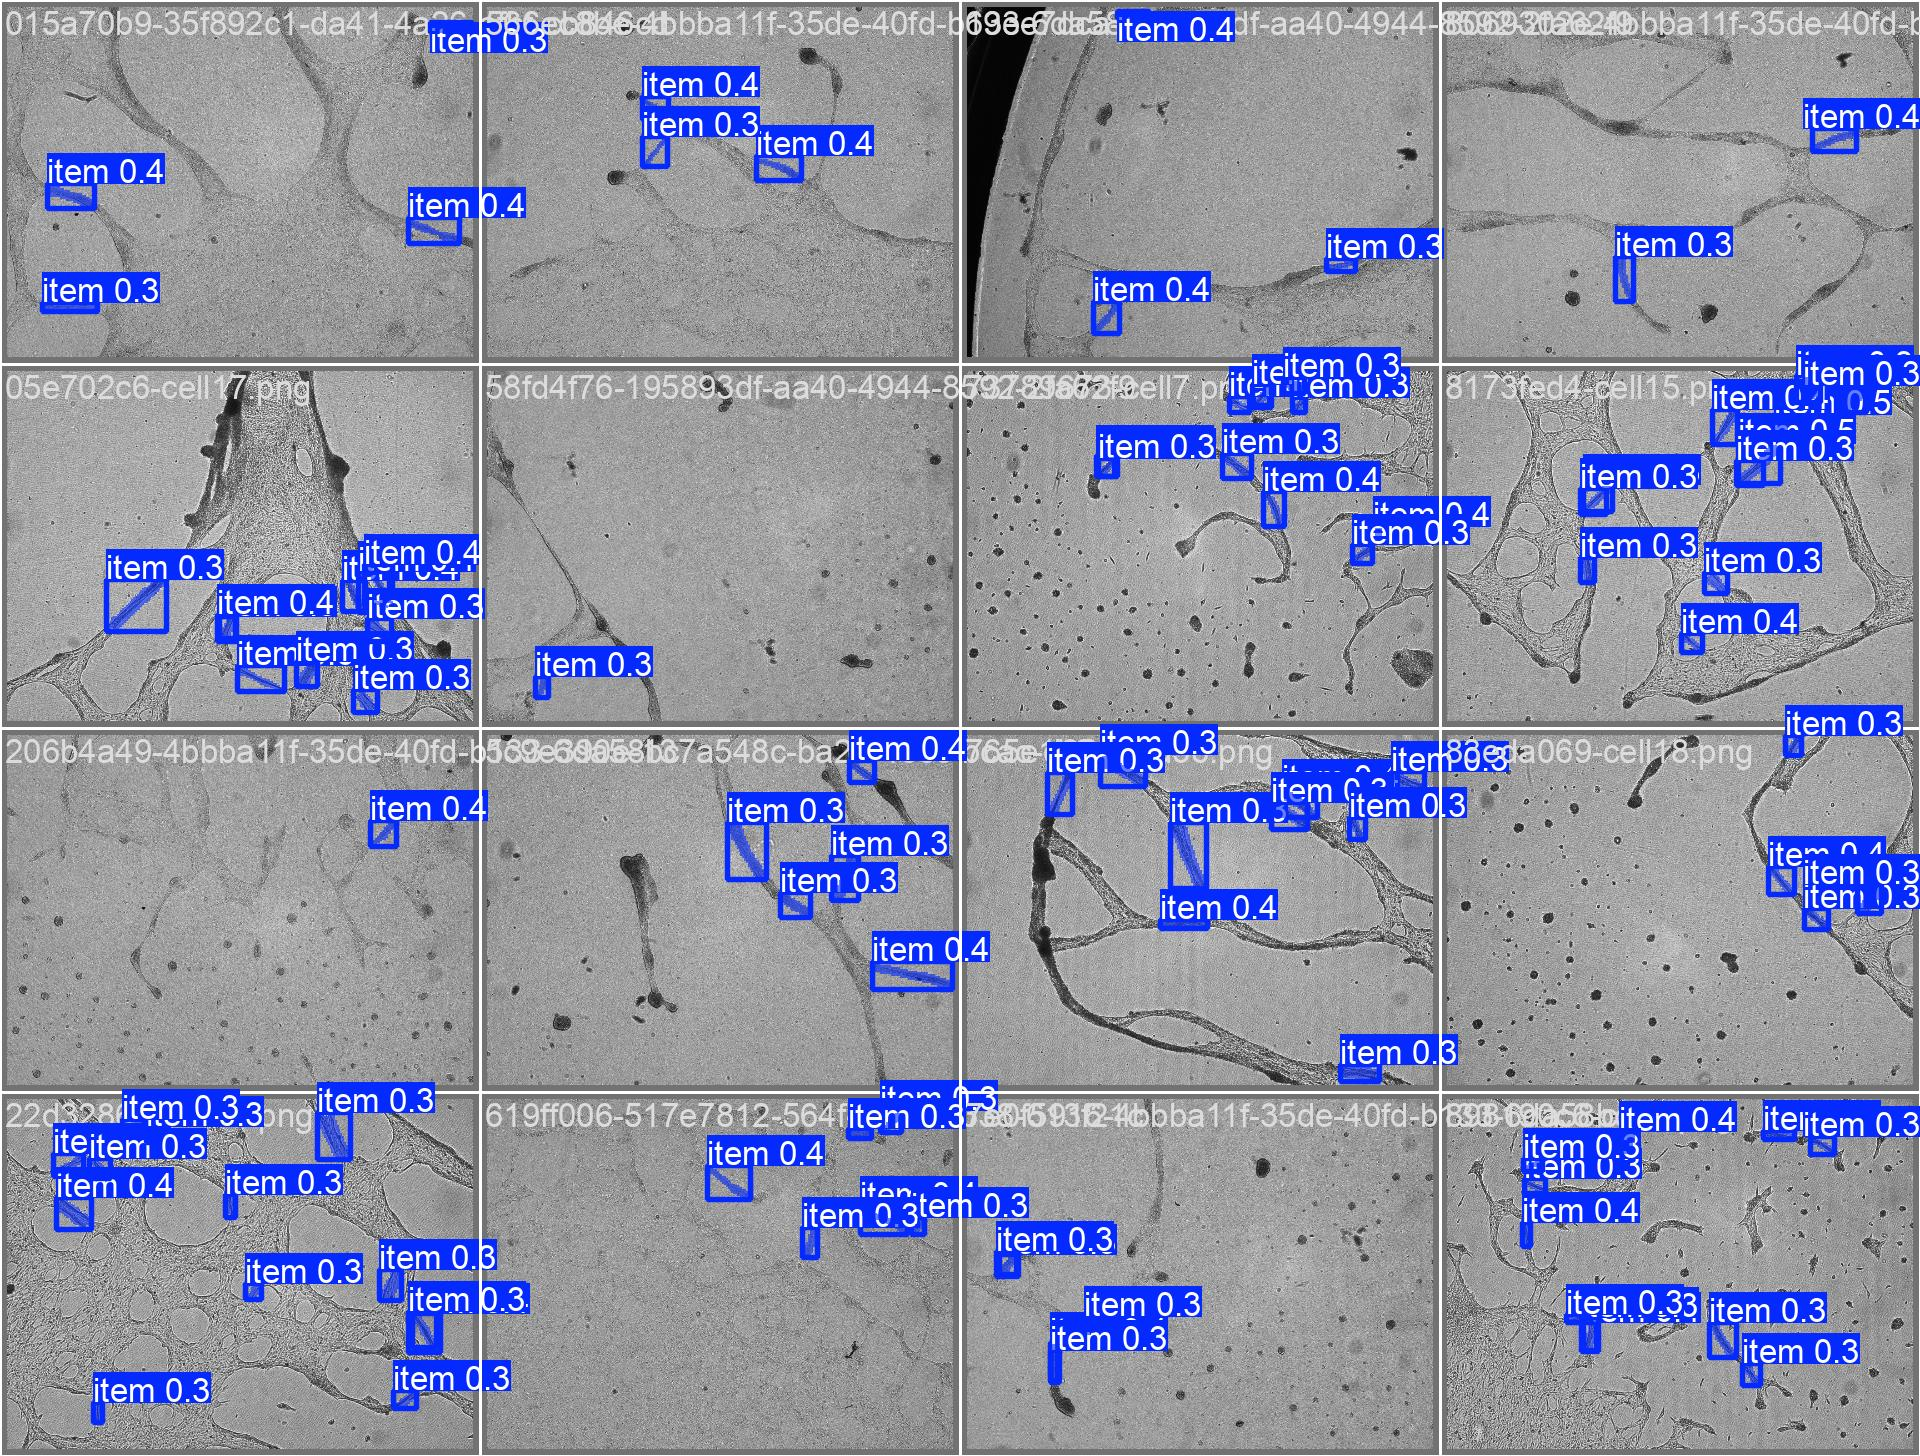
\includegraphics[width=\linewidth]{yolo_finetune_val_pred.jpg}
\captionof{figure}{Predicción fine-tune.}
\end{minipage}
\end{figure}

Las curvas y predicciones muestran contornos incompletos y detecciones fragmentadas. Estos errores coinciden con la baja proporción de miotubo y la variación de apariencia.

\section{Comparación clásica frente a deep learning}

El clasificador de píxeles y YOLO usan unidades de evaluación distintas. El clasificador informa métricas píxel a píxel en validación, mientras YOLO informa detección de máscaras, precisión y recall de instancia, junto con mAP. Las cifras no son intercambiables sin una evaluación conjunta. Incluso así, permiten una comparación inicial cuando se añaden puntuaciones compatibles.

\begin{table}[H]
\centering
\small
\caption{Comparación inicial de enfoques sobre validación.}
\begin{tabular}{lrrrr}
\toprule
Modelo & Dice píxel & IoU píxel & Precisión & Recall\\
\midrule
HGB clásico & 0.2832 & 0.1650 & 0.3084 & 0.2618\\
YOLO transferencia & No disponible & No disponible & 0.4574 & 0.4690\\
YOLO fine-tune & No disponible & No disponible & 0.4891 & 0.5379\\
\bottomrule
\end{tabular}
\end{table}

El HGB obtiene 0.2832 de Dice y 0.1650 de IoU a nivel píxel. YOLO no registra esos resultados con la misma máscara binaria en los informes disponibles. Su precisión y recall de máscaras son mayores que los del clasificador, especialmente en fine-tune. Fine-tune alcanza además 0.4763 de mAP50 y 0.1692 de mAP50-95, frente a 0.4364 y 0.1596 en transferencia.

La comparación indica que el enfoque clásico es una línea base útil y económica. Produce métricas por píxel claras, pero su recall permanece bajo y no aprovecha patrones espaciales ni contextuales complejos. YOLO ofrece mejores precisión y recall de máscara y su fine-tune supera a la variante con capas congeladas.

Se recomienda continuar con deep learning como dirección principal. Esta decisión debe mantenerse provisional hasta calcular para YOLO el Dice píxel, el IoU píxel y otras métricas por imagen con el mismo conjunto de validación y umbrales del HGB. También conviene evaluar el conjunto de prueba antes de descartar el enfoque clásico. HGB puede conservarse como referencia y como posible modelo de apoyo o validación rápida.

\section{Discusión y conclusiones}

La partición agrupada fue necesaria para evitar que réplicas visuales inflaran los resultados. Las máscaras vacías requieren revisión antes de tratarlas como negativos reales.

El clasificador HGB supera a la línea clásica en PR-AUC, ROC-AUC e IoU. Fine-tune supera a transferencia en los indicadores máximos de máscara. Los resultados siguen siendo insuficientes para uso clínico o automático.

Conviene evaluar el conjunto de prueba, revisar anotaciones inconsistentes y analizar el rendimiento por imagen y tipo de morfología antes de seleccionar un modelo final.

\section{Reproducibilidad}

La partición usa semilla 42 y está registrada en \texttt{data/processed/splits}. Los parámetros YOLO están en sus archivos \texttt{args.yaml}. El conjunto de figuras utilizado se encuentra en \texttt{figures/}.

\end{document}
